%!TEX program = xelatex
\documentclass[12pt, a4paper]{article}

\usepackage[dvipsnames]{xcolor}

\usepackage{fancyhdr}
\usepackage{extramarks}
\usepackage{amsmath}
\usepackage{amsthm}
\usepackage{amsfonts}
\usepackage{tikz}
\usepackage[plain]{algorithm}
\usepackage{algpseudocode}

\usepackage{ctex}
\usepackage{indentfirst}
\usepackage{wrapfig}
\usepackage{upgreek}
\usepackage{subfigure}
\ctexset {today=old}
\usetikzlibrary{automata,positioning,shapes.geometric,arrows.meta,patterns,calc}
\numberwithin{equation}{section}

%
% Basic Document Settings
%

\topmargin=-0.45in
\evensidemargin=0in
\oddsidemargin=0in
\textwidth=6.5in
\textheight=9.0in
\headsep=0.25in

\linespread{1.1}

\pagestyle{fancy}
\lhead{\hmwkAuthorName}
\chead{\hmwkClass\ (\hmwkClassInstructor\ \hmwkClassTime): \hmwkTitle}
\rhead{\firstxmark}
\lfoot{\lastxmark}
% \cfoot{\thepage}
\renewcommand\headrulewidth{0.4pt}
\renewcommand\footrulewidth{0.4pt}

\setlength{\parindent}{2em}  % 2em代表首行缩进两个字符

%
% Create Problem Sections
%

\newcommand{\enterProblemHeader}[1]{
    \nobreak\extramarks{}{Problem \arabic{#1} continued on next page\ldots}\nobreak{}
    \nobreak\extramarks{Problem \arabic{#1} (continued)}{Problem \arabic{#1} continued on next page\ldots}\nobreak{}
}

\newcommand{\exitProblemHeader}[1]{
    \nobreak\extramarks{Problem \arabic{#1} (continued)}{Problem \arabic{#1} continued on next page\ldots}\nobreak{}
    \stepcounter{#1}
    \nobreak\extramarks{Problem \arabic{#1}}{}\nobreak{}
}

\setcounter{secnumdepth}{0}
\newcounter{partCounter}
\newcounter{homeworkProblemCounter}
\setcounter{homeworkProblemCounter}{1}
\nobreak\extramarks{Problem \arabic{homeworkProblemCounter}}{}\nobreak{}

%
% Homework Problem Environment
%
% This environment takes an optional argument. When given, it will adjust the
% problem counter. This is useful for when the problems given for your
% assignment aren't sequential. See the last 3 problems of this template for an
% example.
%
\newenvironment{homeworkProblem}[1][-1]{
    \ifnum#1>0
        \setcounter{homeworkProblemCounter}{#1}
    \fi
    \section{Problem \arabic{homeworkProblemCounter}}
    \setcounter{partCounter}{1}
    \enterProblemHeader{homeworkProblemCounter}
}{
    \exitProblemHeader{homeworkProblemCounter}
}

%
% Homework Details
%   - Title
%   - Due date
%   - Class
%   - Section/Time
%   - Instructor
%   - Author
%

\newcommand{\hmwkTitle}{单元测试错题集}
\newcommand{\hmwkDueDate}{April 3, 2025}
\newcommand{\hmwkClass}{}
\newcommand{\hmwkClassTime}{大学物理}
\newcommand{\hmwkClassInstructor}{}
\newcommand{\hmwkAuthorName}{{\kaishu 魏崃} \(\left|\right.\) 2024302082051}

%
% Title Page
%

\title{
    \vspace{2in}
    \textmd{\textbf{\hmwkTitle}}\\
    \normalsize\vspace{0.1in}\small{Due\ on\ \hmwkDueDate}\\
    \vspace{0.1in}\large{\textit{\hmwkClassInstructor\ \hmwkClassTime}}
    \vspace{3in}
}

\author{\hmwkAuthorName}
\date{}

\renewcommand{\part}[1]{\textbf{\large Part \Alph{partCounter}}\stepcounter{partCounter}\\}

%
% Various Helper Commands
%

% Useful for algorithms
\newcommand{\alg}[1]{\textsc{\bfseries \footnotesize #1}}

% For derivatives
% \newcommand{\deriv}[1]{\frac{\mathrm{d}}{\mathrm{d}x} (#1)}

% For partial derivatives
\newcommand{\pderiv}[2]{\frac{\partial #1}{\partial #2}}

% Integral dx
\newcommand{\dx}{\mathrm{d}x}

% Alias for the Solution section header
\newcommand{\solution}{\textbf{\large Solution}}

% Probability commands: Expectation, Variance, Covariance, Bias
\newcommand{\E}{\mathrm{E}}
\newcommand{\Var}{\mathrm{Var}}
\newcommand{\Cov}{\mathrm{Cov}}
\newcommand{\Bias}{\mathrm{Bias}}


% 我的newcommand
\newcommand{\degree}{^{\circ}}
\newcommand{\arrow}{-{Stealth[length=4mm,width=2mm]}}
\newcommand{\rmd}{\mathrm{~d}}
\newcommand{\deriv}[2]{\frac{\rmd #1}{\rmd #2}}
\renewcommand{\parallel}{\mathrel{/\mskip-2.5mu/}}

\begin{document}

\cfoot{}
\maketitle

\newpage
\mbox{}
\newpage

\pagebreak

% 设置页码格式是阿拉伯数字
\pagenumbering{arabic}
\cfoot{\thepage}

\begin{homeworkProblem}
    
    一质点在$xy$平面内做曲线运动,其任意时刻的位置矢量为$\overrightarrow{r}=\overrightarrow{r}(x, y)$,$s$代表路程,
    $\overrightarrow{v}$表示质点的速度,$\overrightarrow{a}$ 表示加速度,则在下述几种表述中完全正确的是$\left(\quad\right)$。

    \begin{enumerate}
        \item $$v=\frac{\mathrm{d} r}{\mathrm{~d} t}=\sqrt{\left(\frac{\mathrm{d} x}{\mathrm{~d} t}\right)^2+\left(\frac{\mathrm{d} y}{\mathrm{~d} t}\right)^2}$$
        \item $$a=\frac{\mathrm{d}^2 r}{\mathrm{~d} t^2}=\sqrt{\left(\frac{\mathrm{d}^2 x}{\mathrm{~d} t^2}\right)^2+\left(\frac{\mathrm{d}^2 y}{\mathrm{~d} t^2}\right)^2}$$
        \item $$\overrightarrow{a}=\frac{\mathrm{d} \overrightarrow{v}}{\mathrm{~d} t}=\frac{\mathrm{d} v_x}{\mathrm{~d} t} i+\frac{\mathrm{d} v_y}{\mathrm{~d} t} j$$
        \item $$v=\frac{|\mathrm{d} \overrightarrow{r}|}{\mathrm{d} t}=\frac{\mathrm{d} s}{\mathrm{~d} t}$$
    \end{enumerate}
    \vspace{1em}

    \textbf{错解}

    3(C)
    \vspace{1em}

    \textbf{正解}

    4(D)
    \vspace{1em}

    \textbf{解析}

    \begin{enumerate}
        \item $r = \sqrt{x^2 + y^2}$是位置矢量的模长,$\dfrac{\mathrm{d}r}{\mathrm{d}t}$表示径向速度(位置矢量模长的变化率)。
            而速率$v$应为速度矢量的模,即\(\sqrt{\left(\dfrac{\mathrm{d}x}{\mathrm{d}t}\right)^2 + \left(\dfrac{\mathrm{d}y}{\mathrm{d}t}\right)^2}\),
            但$\dfrac{\mathrm{d}r}{\mathrm{d}t} \neq v$(除非质点沿径向运动)。例如,圆周运动时$\dfrac{\mathrm{d}r}{\mathrm{d}t}=0$,但速率$v \neq 0$。因此选项1错误。
        \item $\dfrac{\mathrm{d}^2 r}{\mathrm{d}t^2}$是位置矢量模长的二阶导数,而加速度大小应为$\sqrt{\left(\dfrac{\mathrm{d}^2x}{\mathrm{d}t^2}\right)^2 + \left(\dfrac{\mathrm{d}^2y}{\mathrm{d}t^2}\right)^2}$。  
            例如,匀速圆周运动中$\dfrac{\mathrm{d}^2r}{\mathrm{d}t^2}=0$,但加速度大小$a = \dfrac{v^2}{r} \neq 0$。因此选项2错误。
        \item 严格来说,选项C的表达式在直角坐标系下是正确的,因为加速度是速度矢量的导数,即:  
            $$
                \overrightarrow{a} = \frac{\mathrm{d}\overrightarrow{v}}{\mathrm{d}t} = \frac{\mathrm{d}v_x}{\mathrm{d}t} \overrightarrow{i} + \frac{\mathrm{d}v_y}{\mathrm{d}t} \overrightarrow{j}
            $$  
            选项3可能未正确使用矢量符号(如标量等式),导致错误。
        \item $|\mathrm{d}\overrightarrow{r}|$是位移矢量的模长微分,即$\mathrm{d}s = |\mathrm{d}\overrightarrow{r}| = \sqrt{(\mathrm{d}x)^2 + (\mathrm{d}y)^2}$,
            因此$\dfrac{|\mathrm{d}\overrightarrow{r}|}{\mathrm{d}t} = \dfrac{\mathrm{d}s}{\mathrm{d}t} = v$,选项4正确。
    \end{enumerate}

\end{homeworkProblem}

% \pagebreak

\begin{homeworkProblem}
    
    一根劲度系数为\(k\)、原长为\(l\)的轻质弹簧,上端悬挂在\(O\)点,下端系一个质量为\(m\)的小球(可视为质点)。
    现给予小球一个水平方向的初速度\(v_0\),使小球在竖直平面内向上摆动。若以小球和弹簧作为一个系统,
    则小球在上摆过程中,下列说法正确的是$\left(\quad\right)$。

    \[
        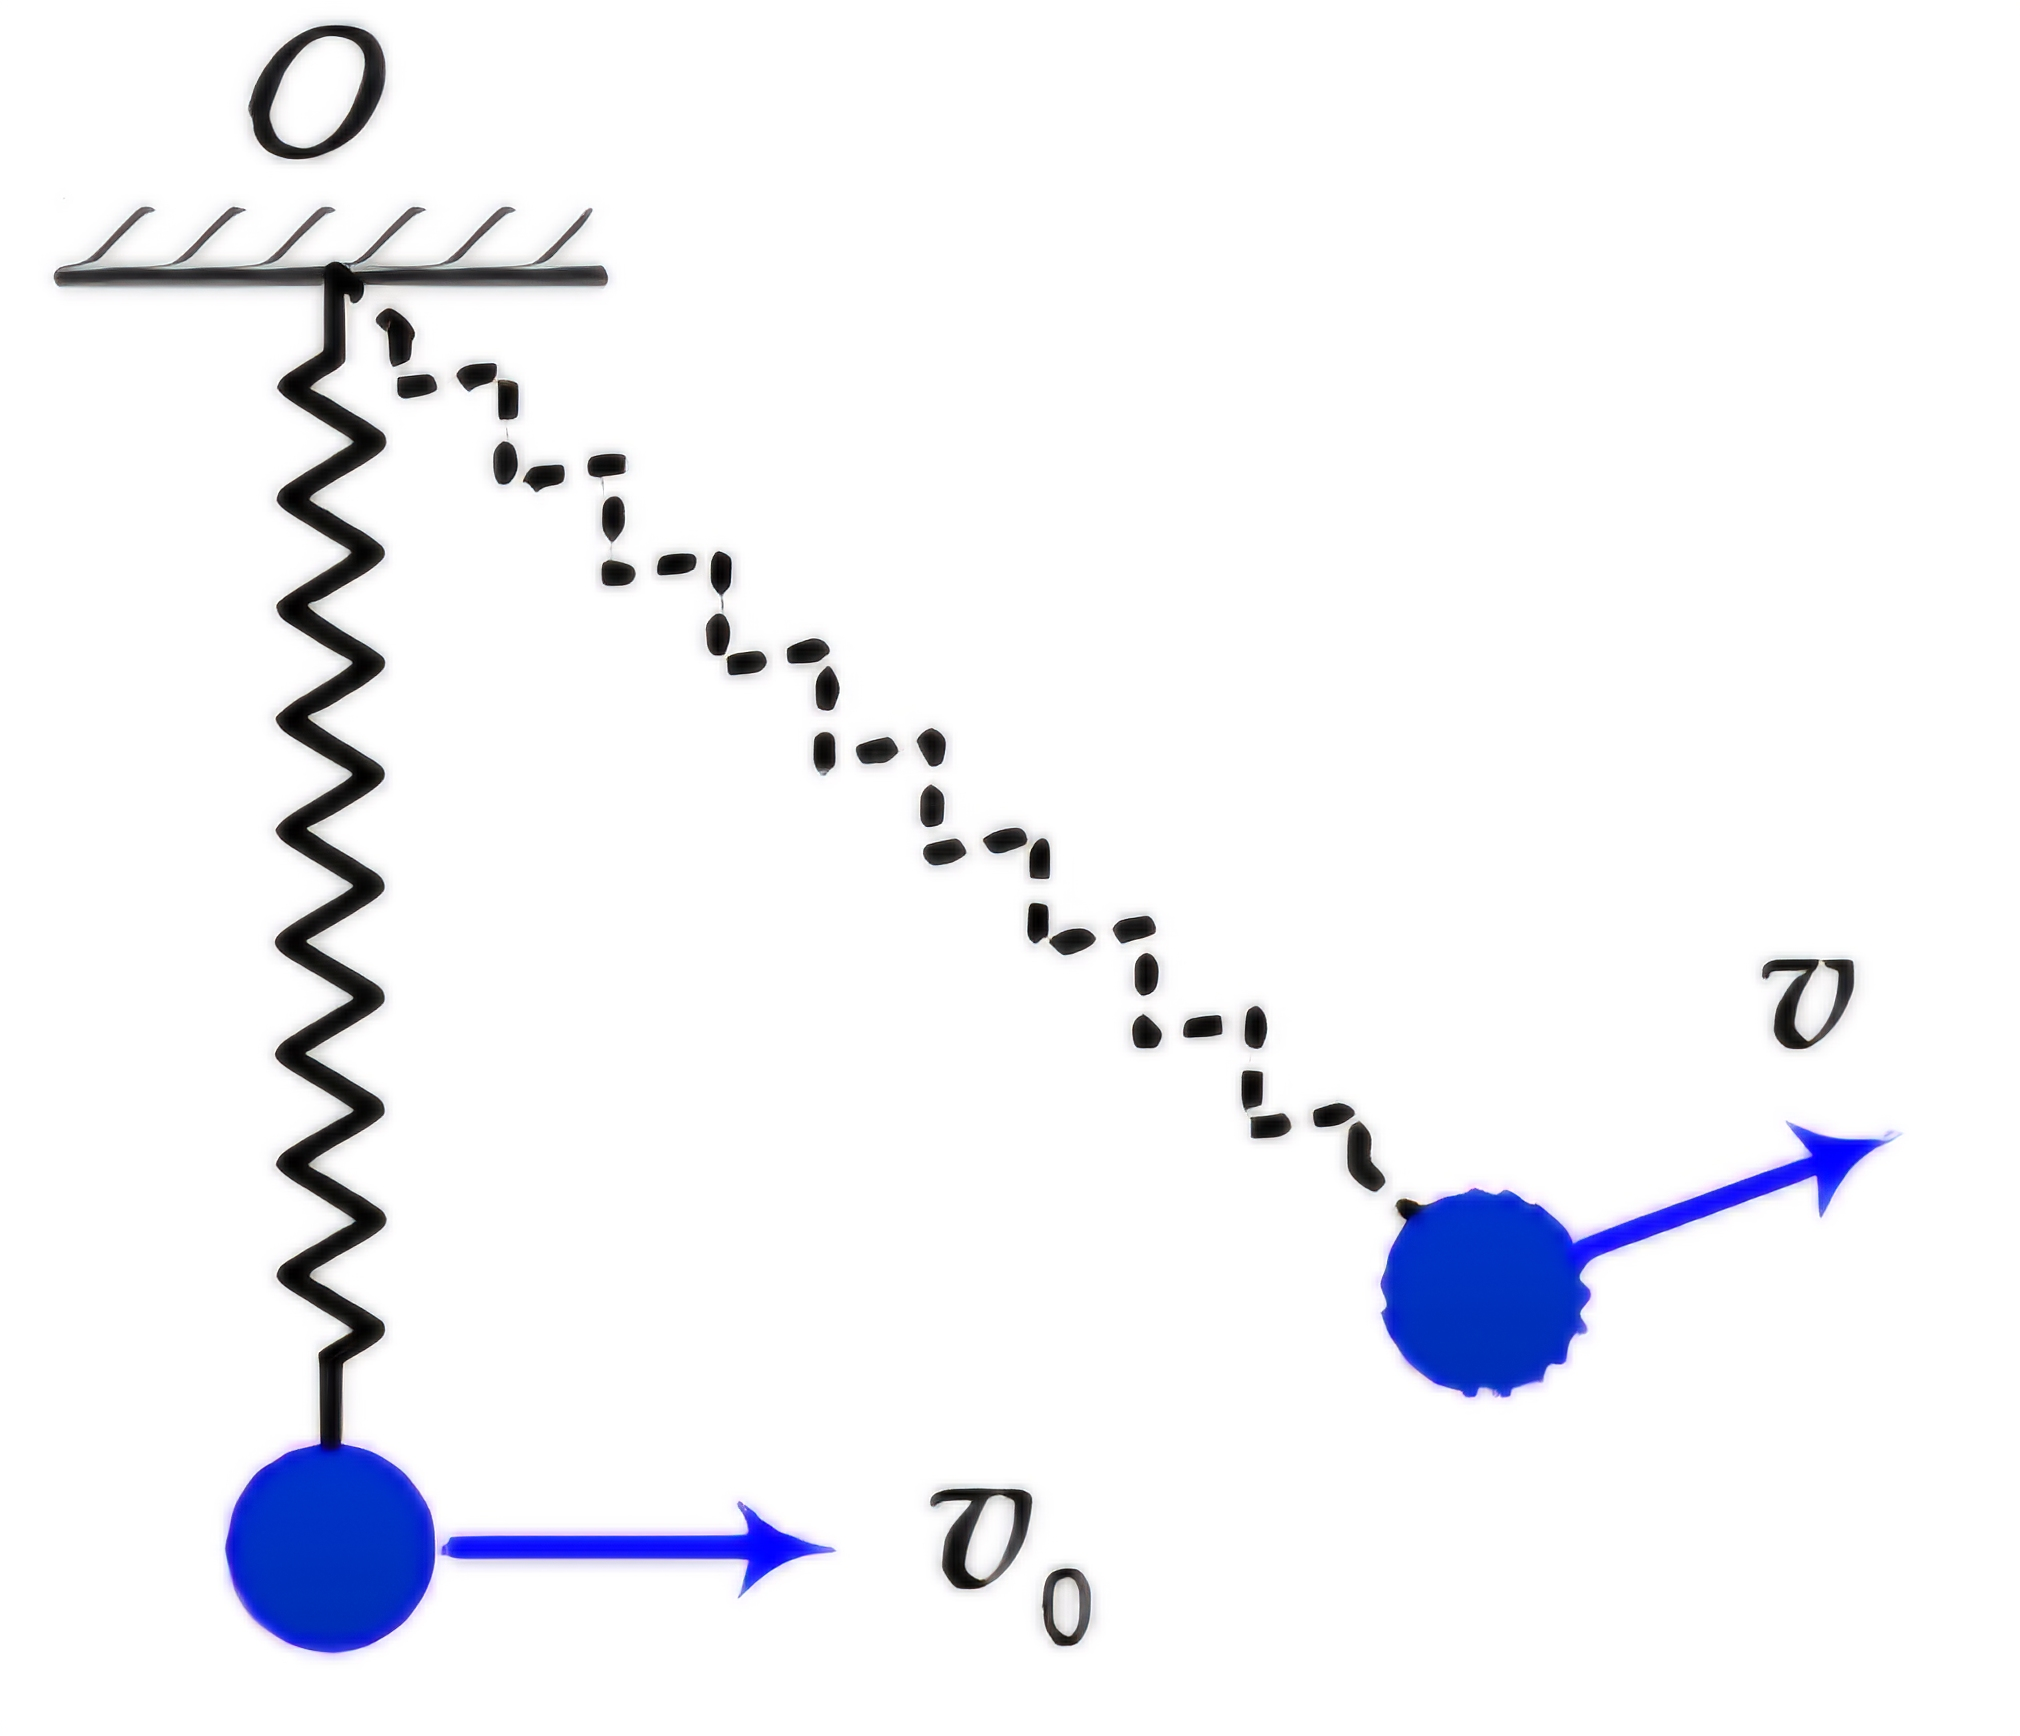
\includegraphics[scale=0.08]{Unit Test Error Collection images/pic1.jpg}
    \]

    \begin{enumerate}
        \item 系统的机械能守恒,系统对\(O\)点的角动量守恒
        \item 系统的机械能不守恒,系统对\(O\)点的角动量守恒
        \item 系统的机械能守恒,系统对\(O\)点的角动量不守恒
        \item 系统的机械能不守恒,系统对\(O\)点的角动量不守恒
    \end{enumerate}
    \vspace{1em}

    \textbf{错解}

    3(C)
    \vspace{1em}

    \textbf{正解}

    4(D)
    \vspace{1em}

    \textbf{解析}

    机械能:系统包括小球和弹簧,但未包括地球。重力作为外部力,做功导致机械能不守恒。
    
    角动量:重力产生的外力矩不为零,导致系统对\(O\)点的角动量不守恒。

\end{homeworkProblem}

\end{document}
